\section{Implementation}

Our system uses input from sensors that inform the controller processor whether a bus or pedestrians are present, and adjust lights accordingly. Therefore, it's a computerized controller in opposition to electromechanical controller in which the logic stands in hardware (dial timer, motor, relays..).

\subsection{Micro-controller}

We had at our disposition Arduino Uno, Arduino Due, Arduino Yun and Intel Galileo board. We choose the Arduino Due because we feared than we might need more I/O pins than other board provide (but in the end it was not the case). Nevertheless, the biggest advantage the Arduino Due provides is that it can deliver way more power on the pin. Thanks to that last advantage, we did not need to use relays and an external power supply.

\subsection{Environment input}

We put two buttons to simulate outside events for bus and pedestrians. We could have used a proximity sensor instead for the bus if we had one available.

\subsubsection{Interruption}

We wired those two button to pins which setup to be attached to an interruption. The rising of current on those pin trigger the interruption. The triggering is done in hardware and its effect is to call a specific function called an Interrupt Service Routine attached during the setup.

\subsubsection{ISR}

In our code the Interrupt Service Routine is only setting a volatile Boolean to true. We purposely wanted to keep the ISR function as small as possible since it's not possible to interrupt an interruption on an Arduino board. Other interruptions during an interruption are simply ignored. That means that if there is a bus call during a pedestrian ISR, the first one would be ignored. That is why we wanted to keep it as small as possible. 

\subsection{From Uppaal to C}

Thanks to Uppaal, we believe to have a correct theoretical model. We have respected the model to make our C code. We can thus see the state and transition in our C code. Here is an extract of it:

\begin{verbatim}
[...]
enum CrosswalkTrafficLightStates { C_GREEN, C_RED, C_CALLED, C_PREEMPTED, C_DELAYEDCALL, C_BUSPATH };
[...]
VehicleTrafficLight trafficLightLeftRight, trafficLightFrontBack;
CrosswalkTrafficLight crosswalk;
BusTrafficLight buspath;
[...]
void trafficLightLeftRightFromRedToGreen() {
    debug("trafficLightLeftRight: Red --> Green");
    trafficLightLeftRight.state = V_GREEN;
    digitalWrite(LEFT_RIGHT_RED, LOW);
    digitalWrite(LEFT_RIGHT_GREEN, HIGH);

}
[...]
void buspathCallISR(){
    isrBuspath = true;
}
[...]
\end{verbatim}


\subsection{Serial monitor}

To be able to detect hardware problems (e.g. disordered button) and follow the execution of our system, we enabled the Arduino Serial Monitor. Here is an example of an execution trace :

\begin{verbatim}
========= RESET =========
verifier() : OKAY
setup() : initialisation done
crosswalkCall() : ISR : button pressed
crosswalk: Red --> Called
SIGNAL: PEDESTRIAN
trafficLightFrontBack: Red --> Crosswalk
SIGNAL: CHANGE
trafficLightLeftRight: Green --> Red
crosswalk: Called --> Green
SIGNAL: PEDESTRIAN
trafficLightLeftRight: Red --> Crosswalk
verifier() : OKAY
SIGNAL: CHANGE
crosswalk: Green --> Red
SIGNAL: FREE
trafficLightLeftRight: Crosswalk --> Red
trafficLightFrontBack: Crosswalk --> Green
verifier() : OKAY
SIGNAL: CHANGE
trafficLightFrontBack: Green --> Red
trafficLightLeftRight: Red --> Green
verifier() : OKAY
\end{verbatim}

\subsection{Redundant checker}

We defined a function that check if there is a conflicting state in our system (e.g. conflicting green lights). It is called at each transition. If it finds something wrong, it proceeds to turnoff all light except a blinking alert LED.


\subsection{Demonstration}

Here is a 2 minutes video that shows what we implemented better than a thousand words description would.

\begin{figure}[H]\label{fig:ytv}
  \centering
    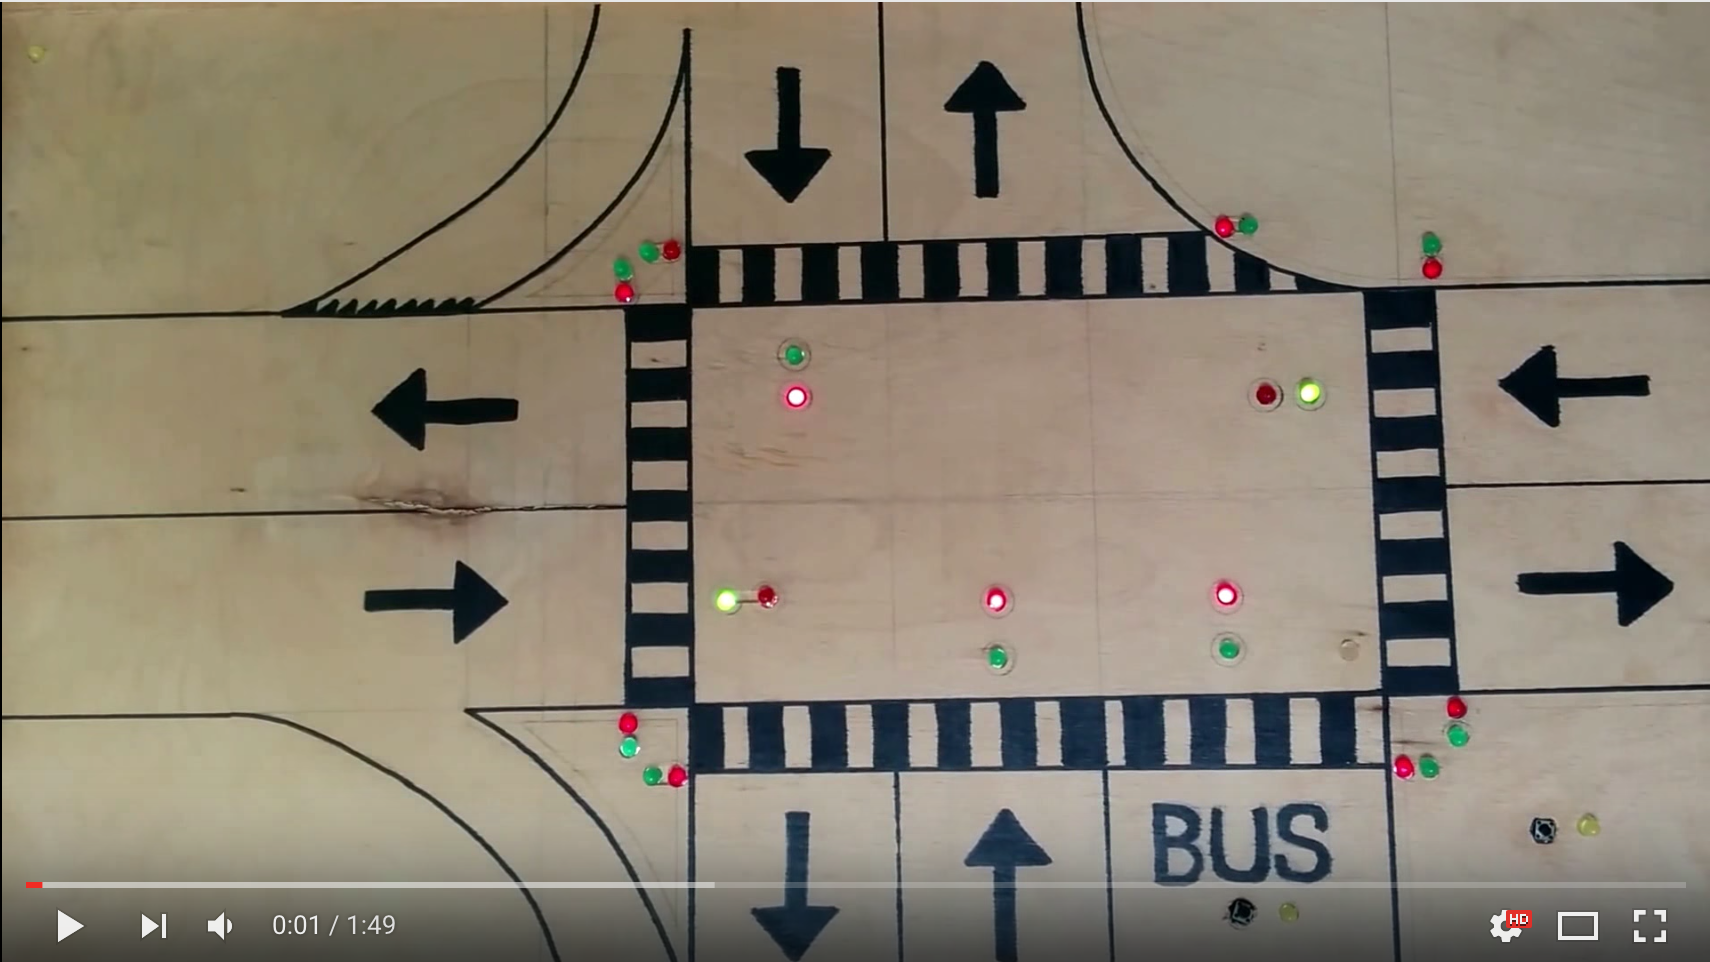
\includegraphics[width=0.7\textwidth]{picture/demo.png}
    \caption{YouTube demonstration}
\end{figure}

It's accessible at :  \url{https://www.youtube.com/watch?v=eleQZ59nWXM}.